\documentclass{beamer}
\usetheme{metropolis}           % Use metropolis theme
\definecolor{goethe_blau}{HTML}{00618F} % define goethe color
%\setbeamercolor{frametitle}{bg=goethe_blau}
\setbeamercolor{alerted text}{fg=goethe_blau} % use goethe color


%\usepackage[
%    backend=biber,
%    style=apa,
%  ]{biblatex}
%\addbibresource{presentation/bibliography.bib}

\titlegraphic{
\includegraphics[width=2.5cm]{presentation/images/GoetheLogo.png}}

%\logo{{
\includegraphics[width=2cm]{presentation/images/GoetheLogo.png}}\hspace*{1cm}}

\usepackage{caption}

\title{Assembly of long, error-prone reads using repeat graphs}
\date{\today}
\author{Mikhail Kolmogorov, Jeffrey Yuan, Yu Lin, and Pavel A. Pevzner}
\institute{Johannes Hausmann, Luis Kress}


\begin{document}
  \maketitle
  
  %\section{First Section}
  
  \begin{frame}{Background}
    \begin{itemize}[<+- | alert@+>]
      \item Assembly: reconstruct target sequence from the reads

      \item Different assemblers, different graph structures (De-Bruijn, Overlap-layout, String)

      \item Repeats $\rightarrow$ assembly fragmentation
      \begin{figure}
        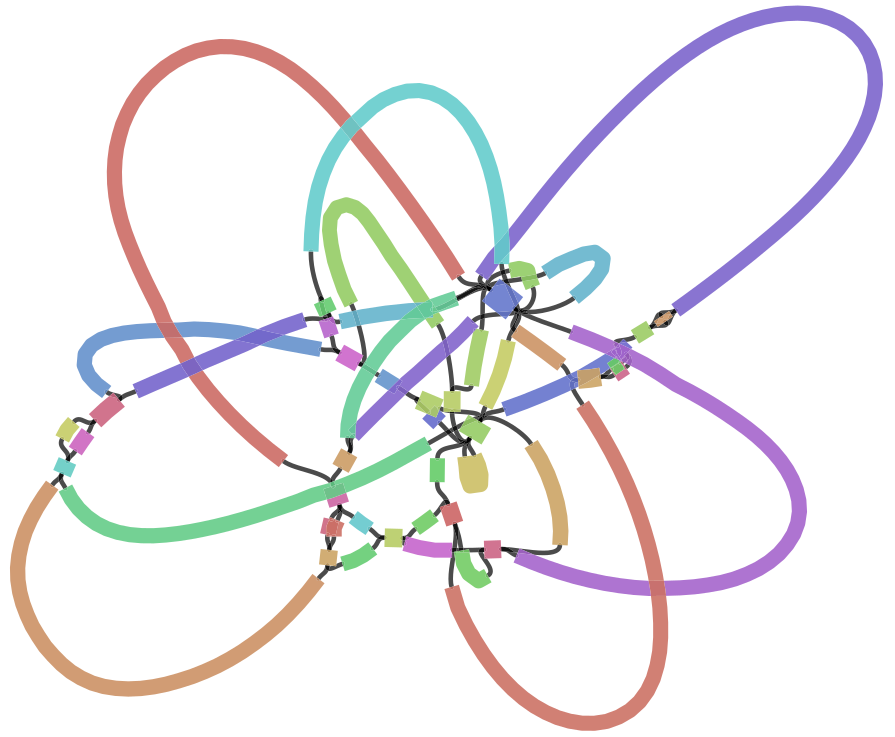
\includegraphics[width=3cm]{presentation/images/tangled.png}
        \caption{Figure 1: Tangled assembly graph\cite{kolmogorov_assembly_2019}}
        \label{fig:tangled}
      \end{figure}

      \item Error rate long read $\leftrightarrow$ short read

      \item Flye $\rightarrow$ resolve these repeats correctly, create contiguous assemblies
    \end{itemize}
  \end{frame}

  %\section{Second Section}

  \begin{frame}{Disjointigs}
    \begin{itemize}[<+- | alert@+>]
      \item Most assemblers spend much time on correct contig assembly

      \item Flye uses a different approach \cite{kolmogorov_assembly_2019}:
      
      \begin{itemize}[<+- | alert@+>]
        \item we don't care \only<4>{(at least at the initial stage)}
        \begin{figure}
          %\captionsetup{labelformat=empty}
          
\includegraphics[width=2.5cm]{presentation/images/orly-owl.jpg}
          %\caption{Orly}
          \label{fig:orly}
        \end{figure}
        
      %  \item correct assembly graph 
      \end{itemize}

      \item Generate paths from overlapping reads without checking for correct repeat resolution $\rightarrow$ Disjointigs
    \end{itemize}
  \end{frame}

  \begin{frame}{Repeat Graph Creation}
    \begin{figure}
      %\captionsetup{labelformat=empty}
      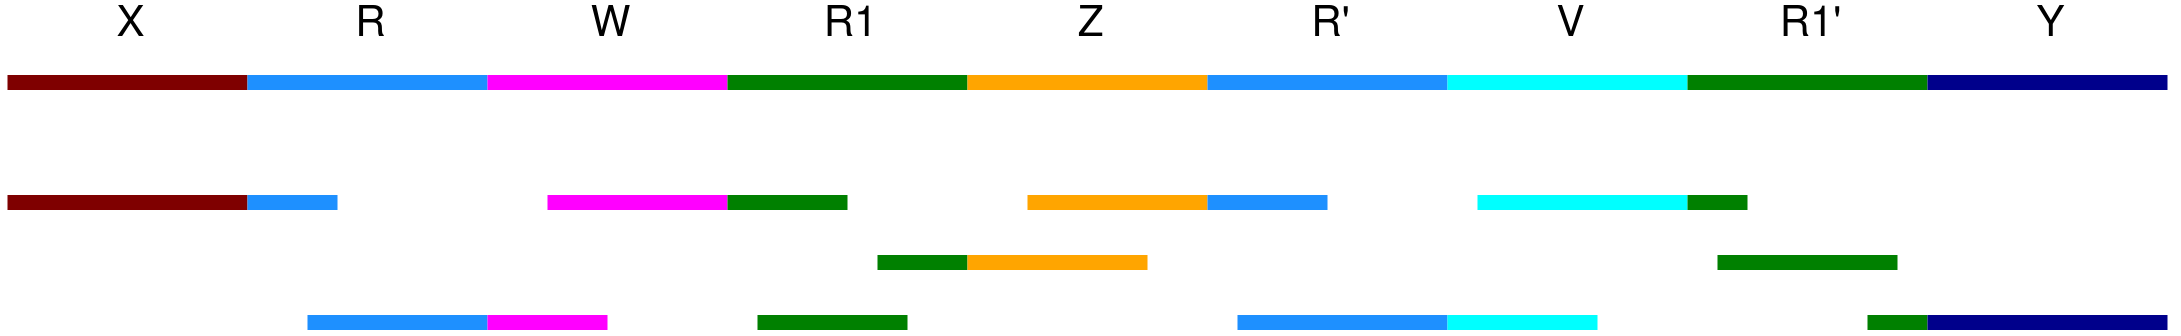
\includegraphics[width=11cm]{presentation/images/genome_and_reads.png}
      %\caption{Example Genome and Reads}
      \label{fig:genome_and_reads}
    \end{figure}
  \end{frame}

  \begin{frame}{Repeat Graph Creation}
    \begin{figure}
      %\captionsetup{labelformat=empty}
      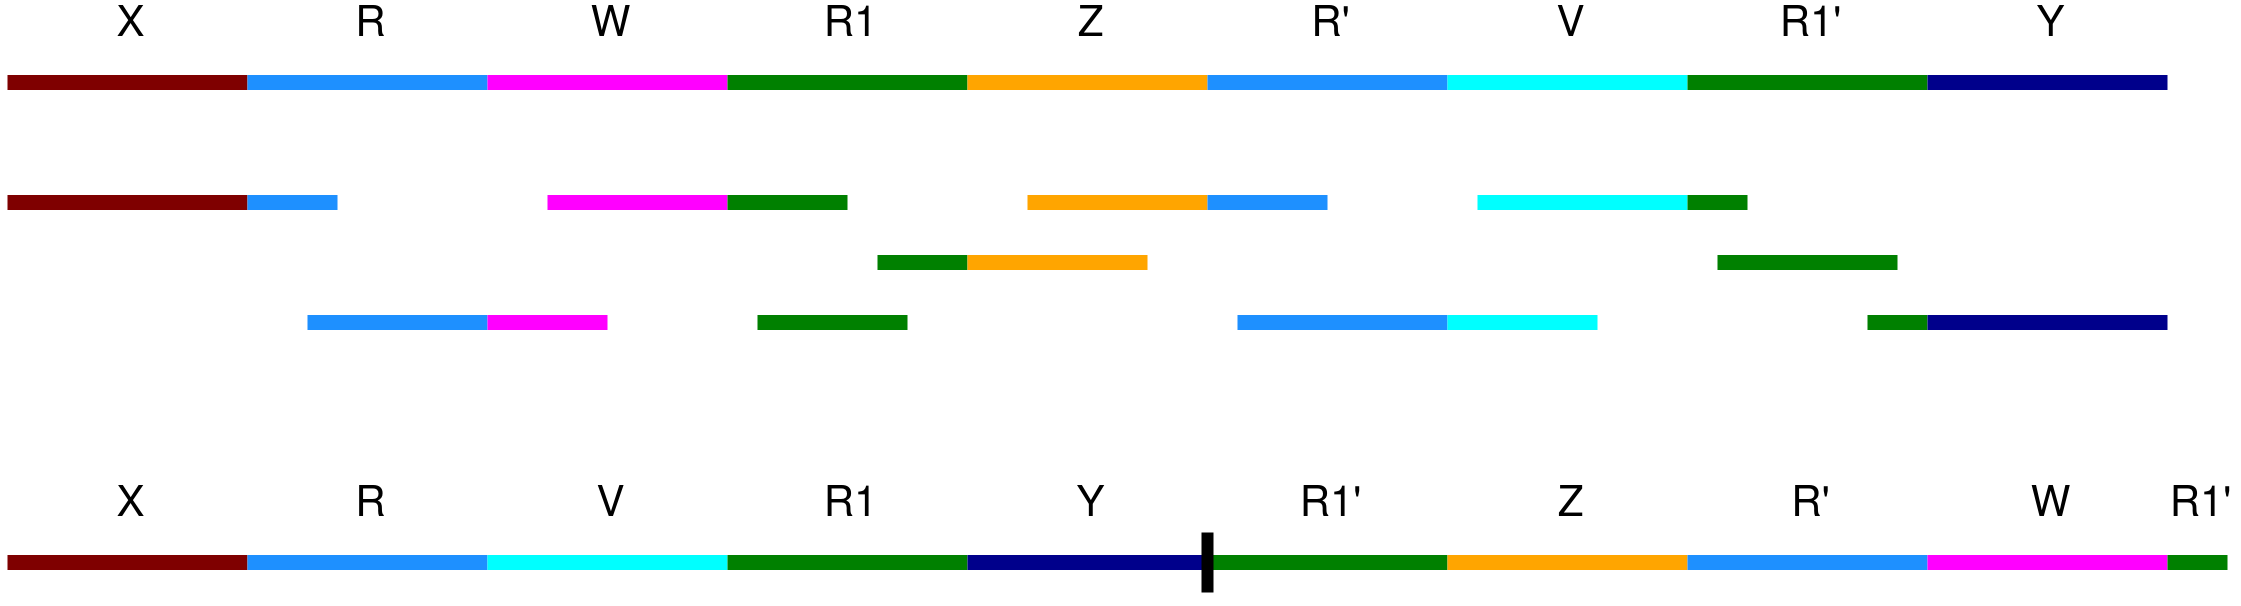
\includegraphics[width=11cm]{presentation/images/disjointigs.png}
      %\caption{Example Genome, Reads and Disjointigs}
      \label{fig:disjointigs}
    \end{figure}
  \end{frame}

  \begin{frame}{Repeat Graph Creation}
    \begin{figure}
      %\captionsetup{labelformat=empty}
      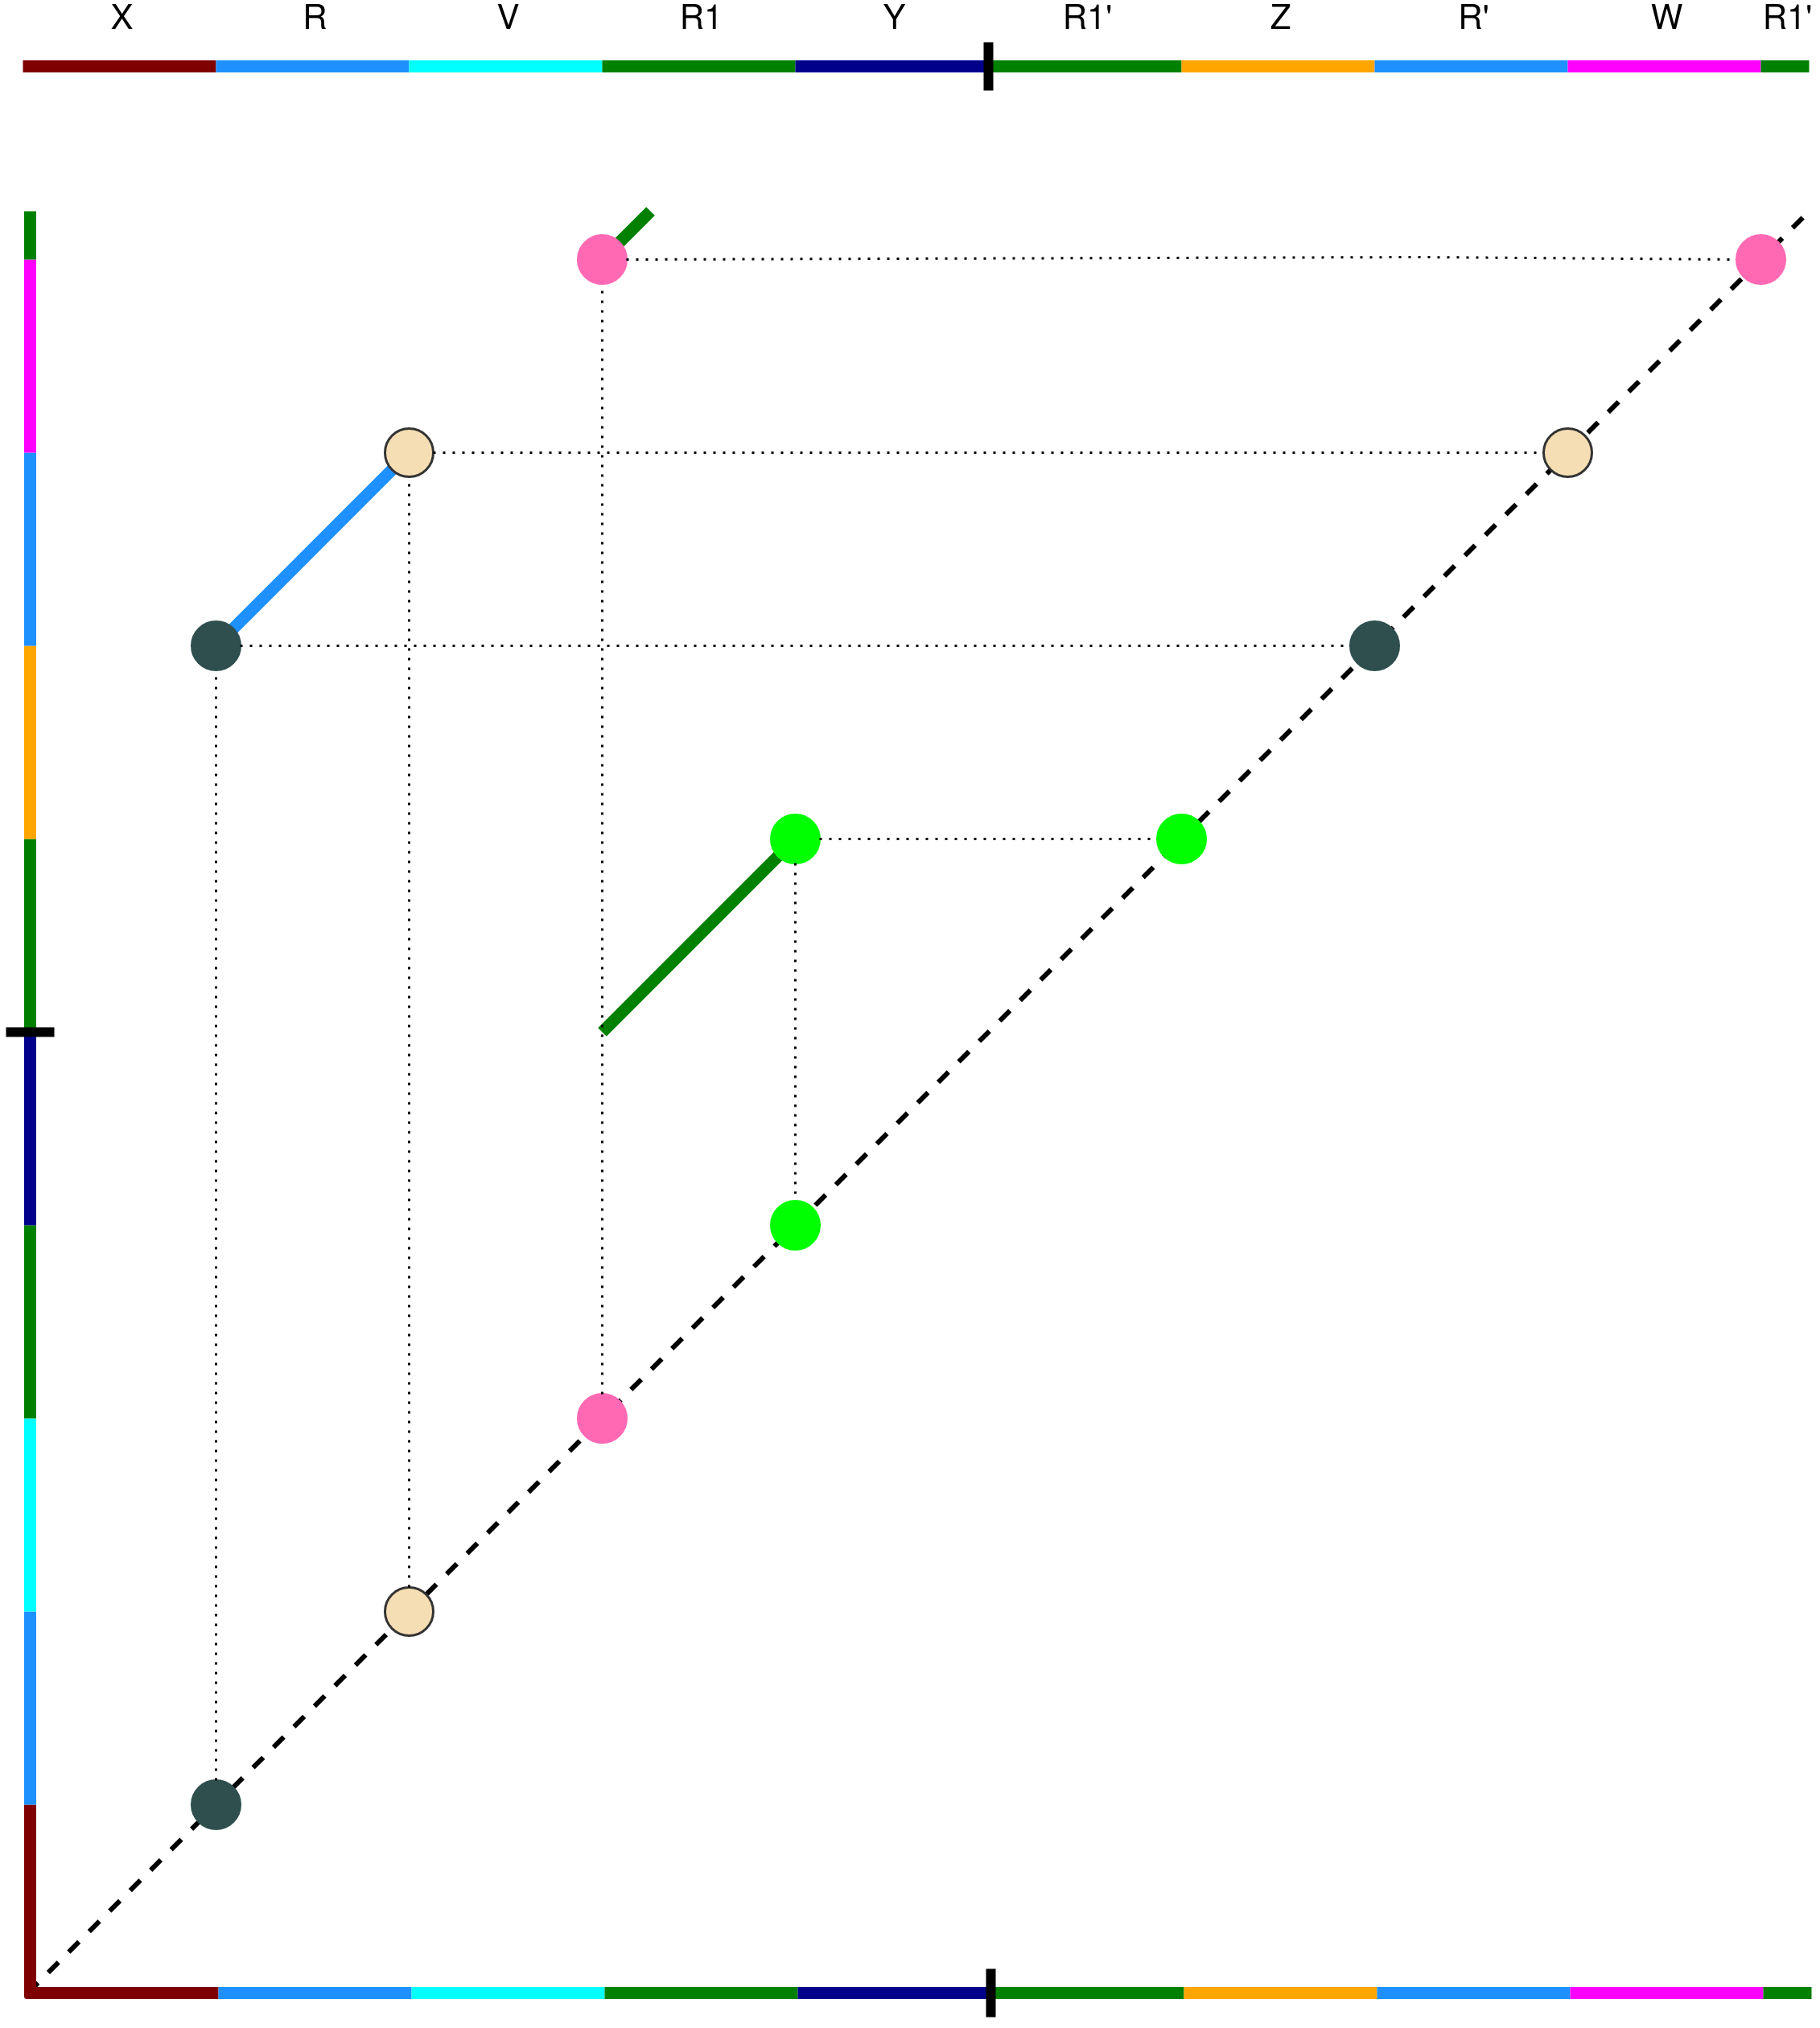
\includegraphics[width=6cm]{presentation/images/dot_plot.png}
      %\caption{Breakpoint Graph}
      \label{fig:bp_graph}
    \end{figure}
  \end{frame}

  \begin{frame}{Repeat Graph Creation}
    \begin{figure}
      %\captionsetup{labelformat=empty}
      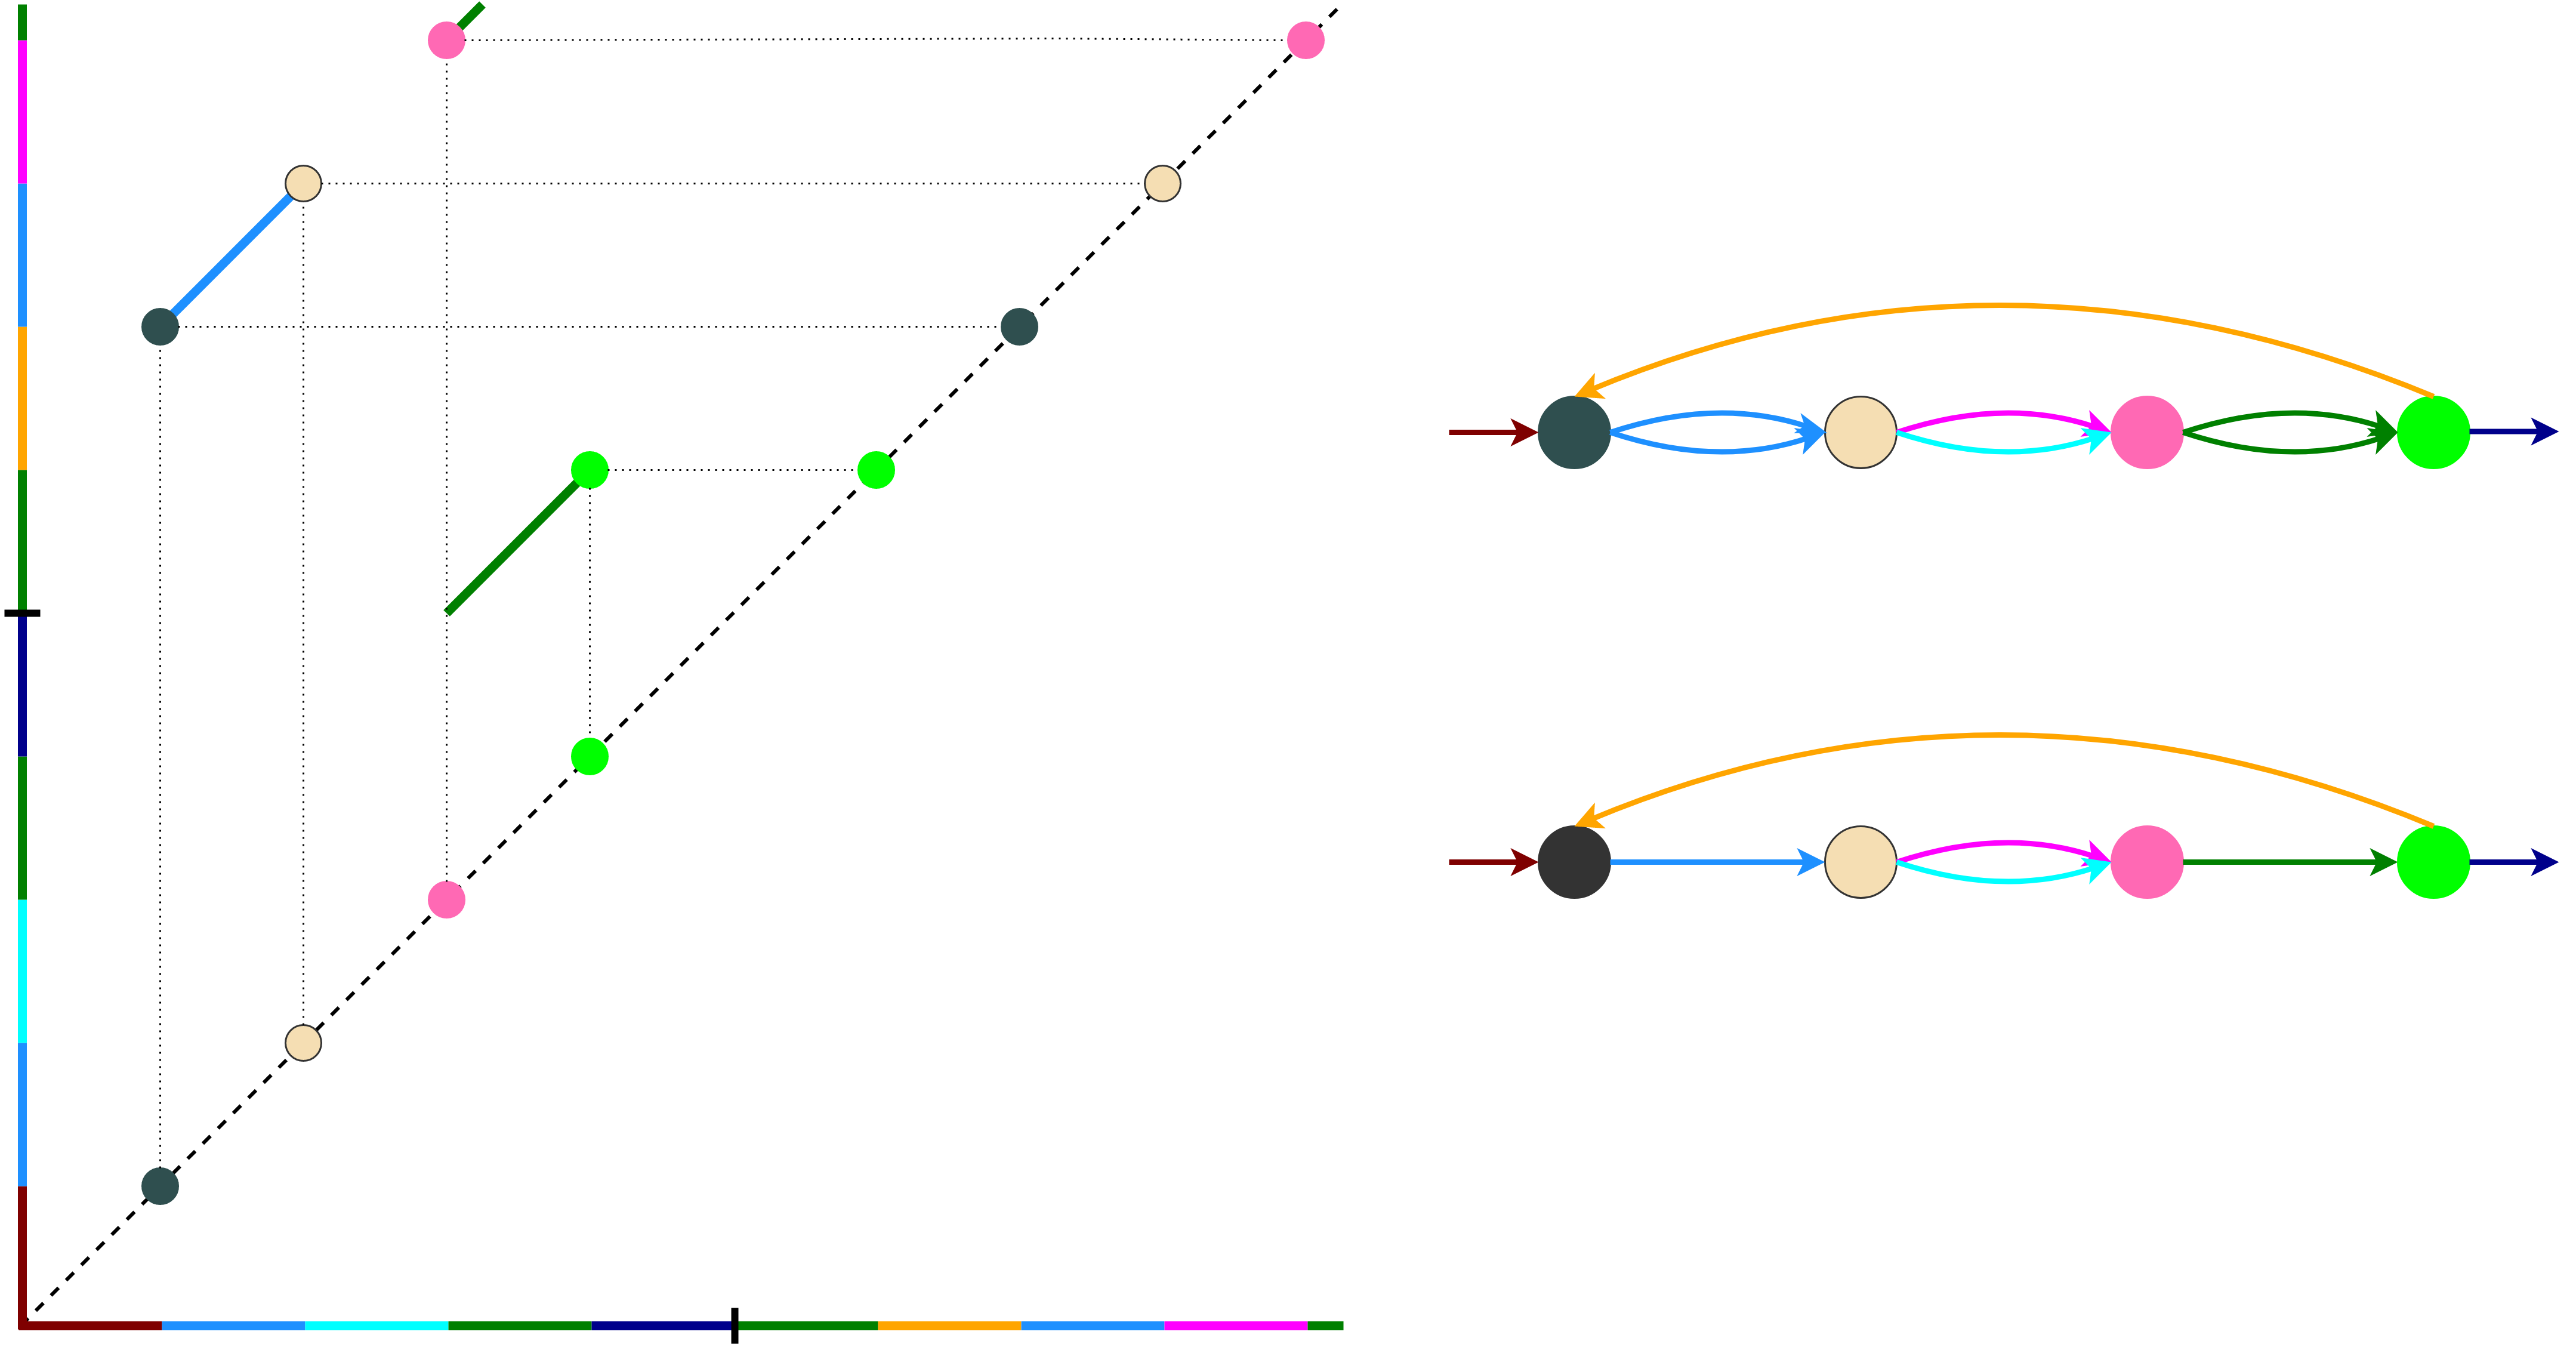
\includegraphics[width=11cm]{presentation/images/plot_to_repeat_graph.png}
      %\caption{Repeat Graph}
      \label{fig:repeat_graph}
    \end{figure}
  \end{frame}

  \begin{frame}{Results}
    \begin{figure}
      \includegraphics[width=11cm]{presentation/images/results_HUMAN.png}
      \caption{Results for HUMAN testset}
      \label{fig:results}
    \end{figure}
  \end{frame}

  \appendix


  \begin{frame}[allowframebreaks]{References}
    %\begin{small} 
    %  dir: \thepwd
    %\end{small}}
    %{\small dir: \thepwd \par}
    
    %\printbibliography
    \bibliography{literature/bibliography.bib}
    \bibliographystyle{abbrv}
  
  \end{frame}

  \begin{frame}{Git (presentation and poster)}

    \begin{figure}
      %\captionsetup{labelformat=empty}
      
\includegraphics[width=6cm]{presentation/images/qr-code.png}
      %\caption{Link to our git repo}
      \label{fig:qr}
    \end{figure}
  
  \end{frame}

  \begin{frame}[standout]
    Appendix
  \end{frame}

  \begin{frame}{Dot plot creation}
    \begin{figure}
      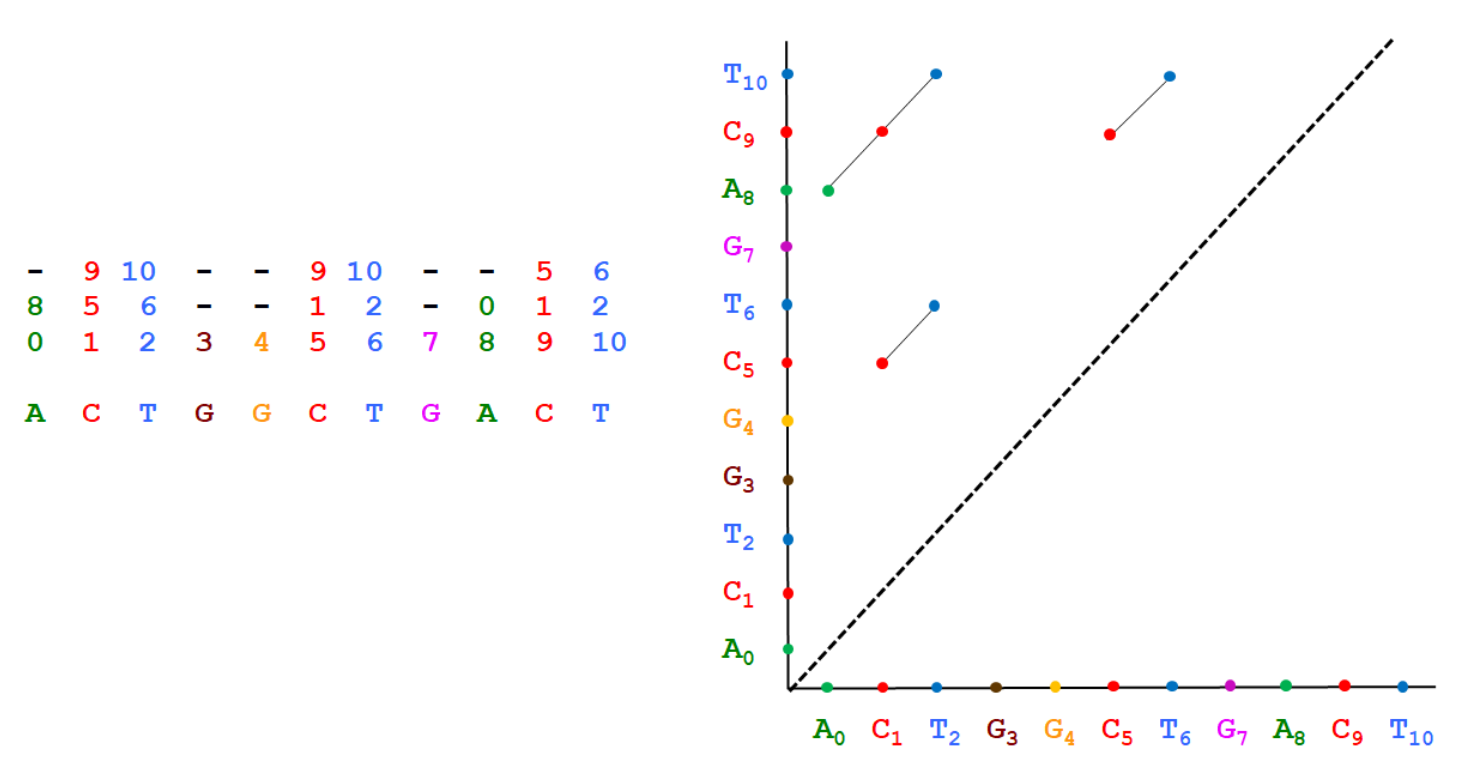
\includegraphics[width=11cm]{presentation/images/dot_plot_creation.png}
      \caption{Dot plot creation}
      \label{fig:dotp_creation}
    \end{figure}
  \end{frame}

  \begin{frame}{Repeat graphs}
    \begin{itemize}
      \item generalization of de bruijn graphs

      \item structure

      \item creation
      
      \begin{itemize}

        \item from disjointigs = random walk of reads on the repeat graph 
      
        \item means the repeat graph hasn't to be known
      \end{itemize}
    \end{itemize}
  \end{frame}

  \begin{frame}{Difference repeat graph de Bruijn graph}
    \begin{itemize}
      \item A-Bruijn graph (alignments) generalizes the de Bruijn graph

      \item We thus argue that the time has come to explain that the breakpoint graphs and the de Bruijn graphs are two identical data structures (if one ignores a cosmetic difference between them) as they both represent specific instances of a general notion of the A-Bruijn graph introduced in [13]. The A-Bruijn graphs are based on representing genomes as sets of labeled paths and further gluing identically labeled edges (breakpoint graphs) or vertices (de Bruijn graphs) in the resulting paths.

      \item de Bruijn graphs need correct bases
      
      \item otherwise tangled graph
    \end{itemize}
  \end{frame}

  \begin{frame}{Segmental duplications}
    \begin{figure}
      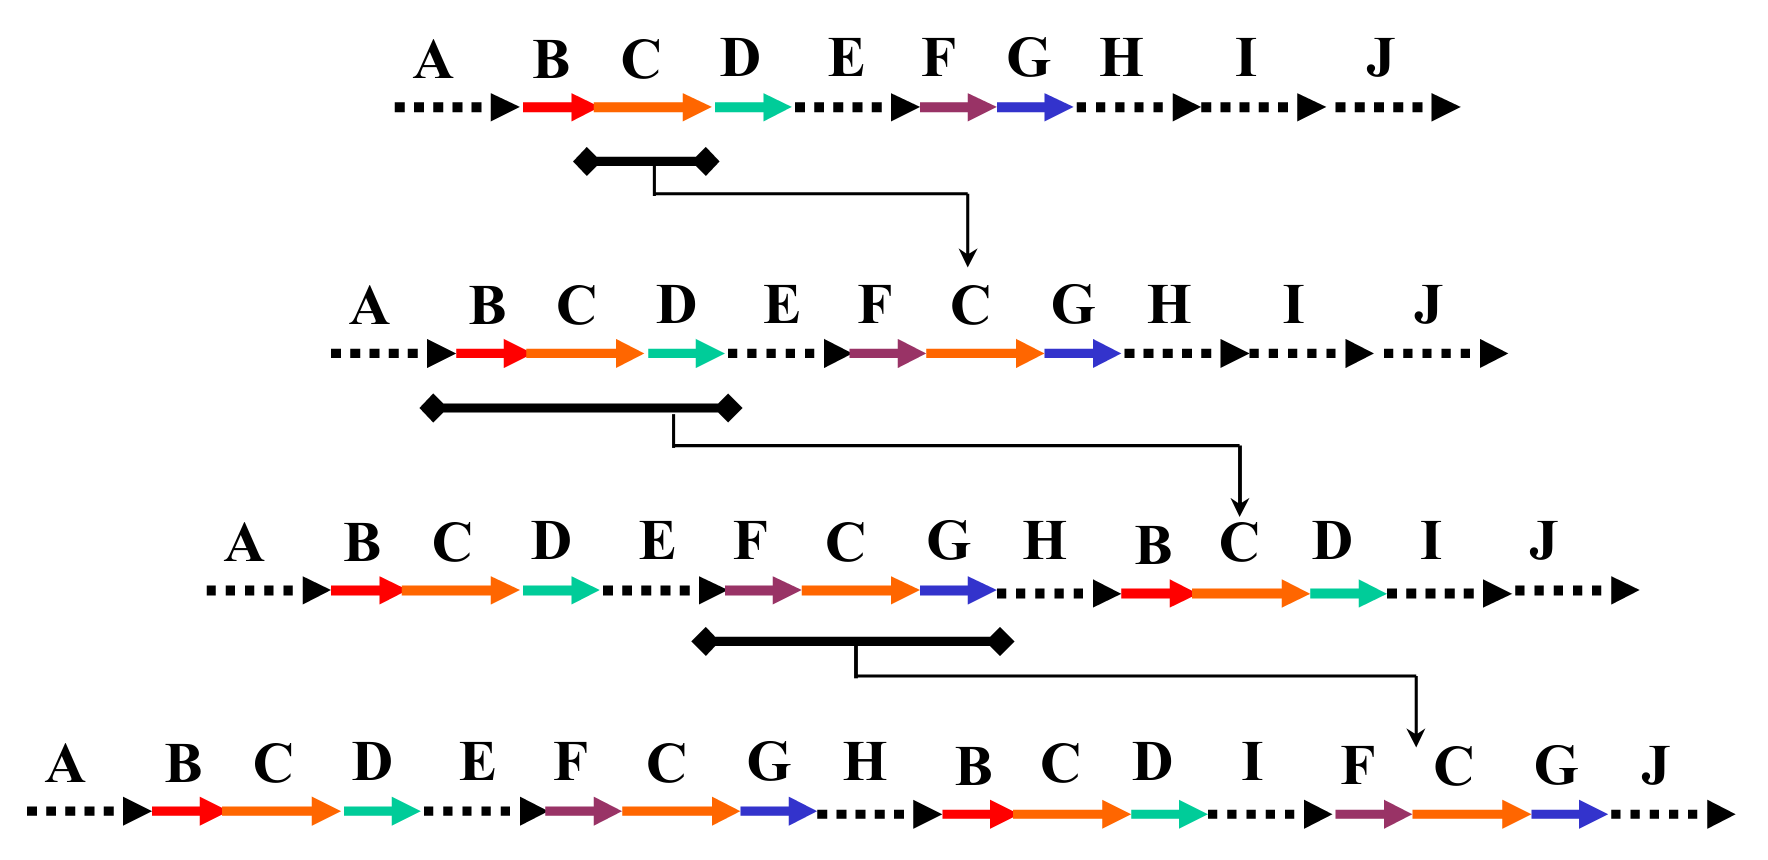
\includegraphics[width=6cm]{presentation/images/SDs.png}
      \caption{Segmental Duplications}
      \label{fig:SD}
    \end{figure}
    \begin{itemize}
      \item Segmental duplications are duplicated blocks of genomic DNA typically ranging in size from 1-200 kb (IHGSC 2001)

      \item They often contain sequence features such as high-copy repeats and gene sequences with intron-exon structure. 
    \end{itemize}
  \end{frame}

  \begin{frame}{Contigity improvement}
    \begin{figure}
      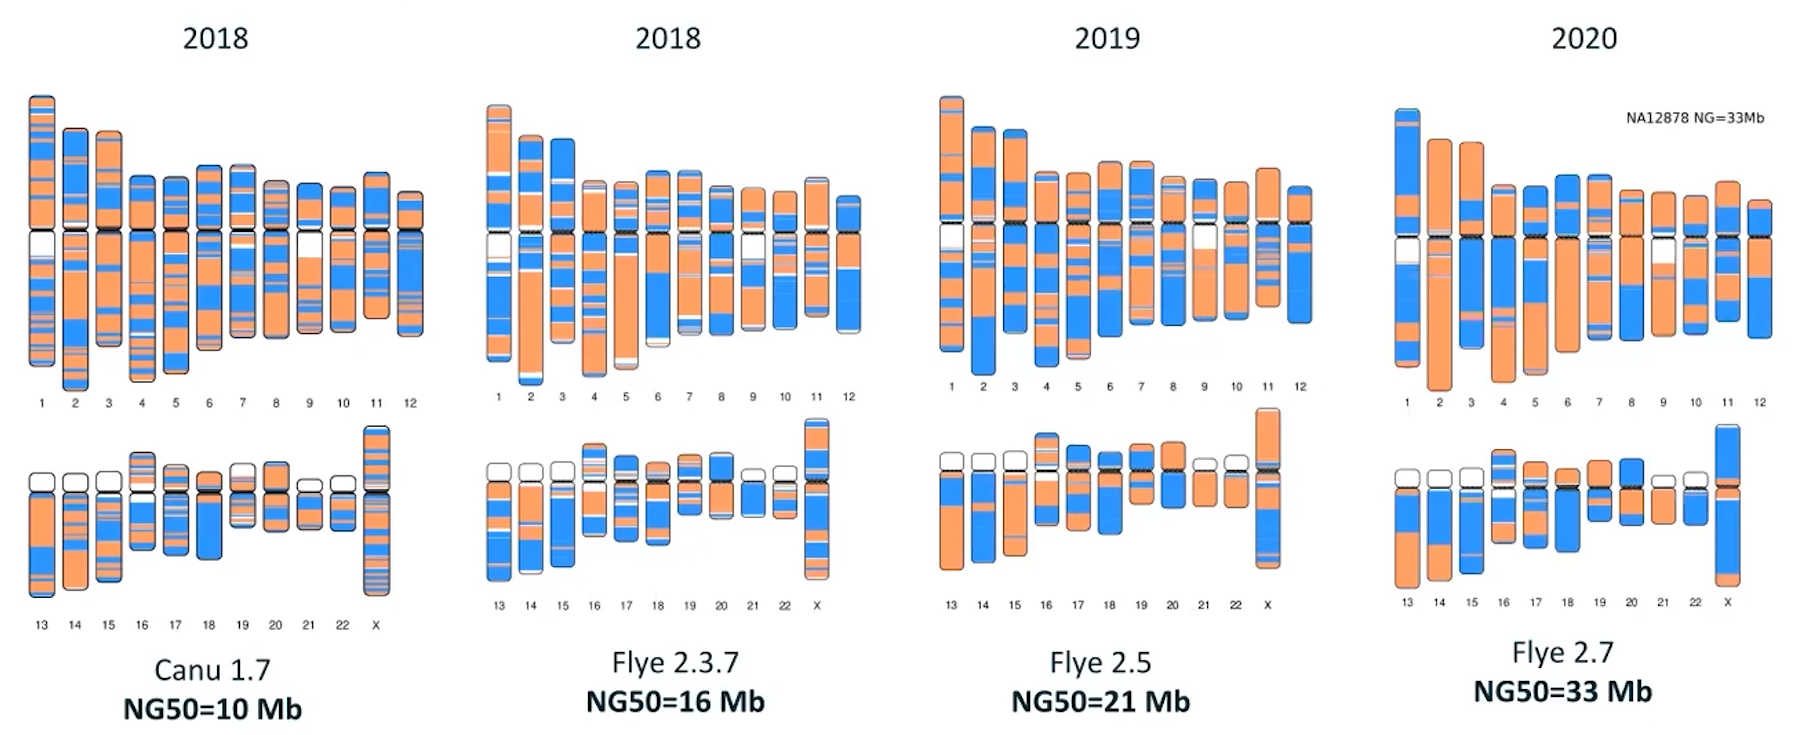
\includegraphics[width=11cm]{presentation/images/contigity_improvement.png}
      \caption{Contigity improvements}
      \label{fig:contig_improvements}
    \end{figure}
    \begin{itemize}
      \item colors are contigs $\rightarrow$ change in color means fragmentation
    \end{itemize}
    %From: 
    %https://www.youtube.com/watch?v=z6elrX-ZzW8&t=636s
    %(Youtube nanopore talk)
  \end{frame}



\end{document}










